\begin{opinion}
%	La causalidad ha sido desarrollada por los seres pensantes como una forma de explicar y por 
%	consiguiente conocer el mundo que lo rodea y actuar transformándolo. Por ello ha sido objeto de estudio a través de la historia del pensamiento humano, habiendo sido objeto de valiosas reflexiones fundamentalmente en el campo de la filosofía. Pero por muchos años continuó siendo	considerada una modalidad cualitativa del pensamiento humano hasta que la llegada de la estadística y algunas deficiencias en el análisis cuantitativo de los datos puso en evidencia la necesidad de desarrollar la causalidad sobre bases cuantitativas como complemento de la correlación y demás procederes estadísticos.
%	
%	El trabajo de diploma que presenta para su defensa el estudiante Antonio Jesús Otaño Barrera introduce, de manera innovadora, recientes resultados sobre la modelación cuantitativa de la causalidad utilizando específicamente modelos estructurales causales acompañados de una implementación con una interfaz amistosa con la cual es posible experimentar diferentes modalidades de la causalidad.
%	 
%	Es de señalar la disciplina y el rigor con el que el estudiante enfrentó la tarea sobre un tema que le era totalmente desconocido y como fue satisfaciendo todos los requisitos que le fueron planteados para su realización. Creemos que el estudiante Antonio Jesús Otaño Barrera ha alcanzado el nivel de profesionalidad que exige alcanzar el título de Lic. en Ciencia de la Computación y por tal motivo solicitamos la calificación de Excelente (5) para su trabajo de diploma.
%	
%	La Habana, 20 de noviembre de 2021.
%	
%	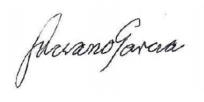
\includegraphics[width=100px, height=80px]{./images/opinion.png}
%	
%	Dr. Luciano García Garrido
%	
%	Profesor Titular Consultante
%	
%	Facultad de Matemática y Computación	
%	
%	Universidad de La Habana, Cuba
	
\end{opinion}